% COMMON RINGS
\newcommand{\N}{\mathbb{N}}
\newcommand{\R}{\mathbb{R}}
\newcommand{\Z}{\mathbb{Z}}
\newcommand{\T}{\mathbb{T}}
\renewcommand{\S}{\mathbb{S}}

% KNOT THEORETIC

% Crossings and singularities
\newcommand*{\double}{\adjustbox{valign=c}{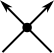
\includegraphics[width=0.05\textwidth]{graphics/glyph_singular_point.pdf}}}
\newcommand*{\poscross}{\adjustbox{valign=c}{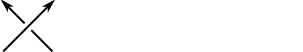
\includegraphics[width=0.05\textwidth]{graphics/glyph_positive_crossing.pdf}}}
\newcommand*{\negcross}{\adjustbox{valign=c}{\includegraphics[width=0.05\textwidth]{graphics/glyph_negative_crossing.pdf}}}


\newcommand*{\tftsouth}{\adjustbox{valign=c}{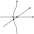
\includegraphics[width=0.11\textwidth]{topological_four_term_south.pdf}}}
\newcommand*{\tfteast}{\adjustbox{valign=c}{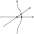
\includegraphics[width=0.11\textwidth]{topological_four_term_east.pdf}}}
\newcommand*{\tftnorth}{\adjustbox{valign=c}{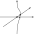
\includegraphics[width=0.11\textwidth]{topological_four_term_north.pdf}}}
\newcommand*{\tftwest}{\adjustbox{valign=c}{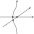
\includegraphics[width=0.11\textwidth]{topological_four_term_west.pdf}}}

\newcommand*{\tot}{\adjustbox{valign=c}{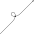
\includegraphics[width=0.11\textwidth]{topological_one_term.pdf}}}

% T4T and T1T (as sums of singular knots)
\newcommand{\tftterm}{\mathbf{T4T}}
\newcommand{\totterm}{\mathbf{T1T}}

% T4T and T1T, DIFF (as relations on invariants)
\newcommand{\tftinv}{\texttt{T4T}}
\newcommand{\totinv}{\texttt{T1T}}
\newcommand{\diffinv}{\texttt{DIFF}}

% T4T and T1T, DIFF (as relations on singular knots)
\newcommand{\tftrel}{\texttt{T4T}\ensuremath{^\ast}}
\newcommand{\totrel}{\texttt{T1T}\ensuremath{^\ast}}
\newcommand{\diffrel}{\texttt{DIFF}\ensuremath{^\ast}}
